\chapter{Experimental results and conclusions}
\section{Results}
Our propose in a nutshell is a new substitutive method of Watershed transform. The following results are obtained using an Acer Aspire E1 laptop with 8 gb of RAM. The figure \ref{fig:alltheprocess} shows all the process starting from the gray scale image to the mask used to find only the leukocytes.
\begin{figure}[htbp]
    \centering
    \begin{subfigure}[b]{0.45\textwidth}
        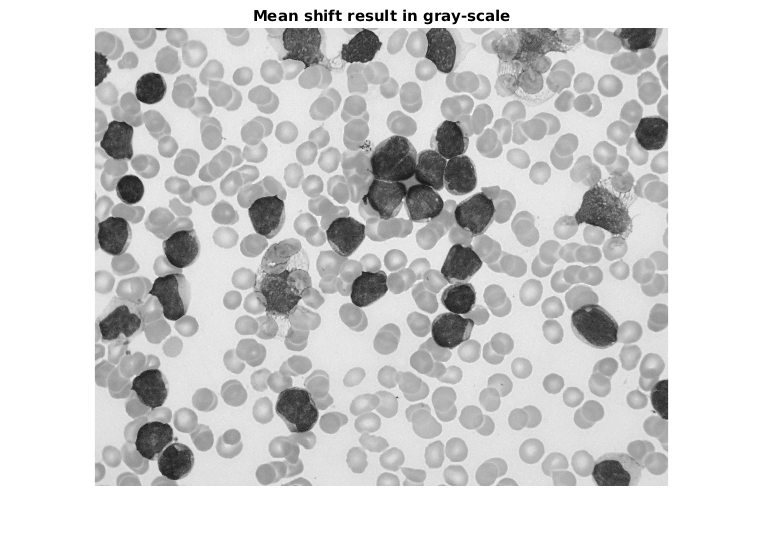
\includegraphics[width=\textwidth]{img/final/figure1.png}
        \caption{ }
        \label{fig:fig1}
    \end{subfigure}
      %(or a blank line to force the subfigure onto a new line)
    \begin{subfigure}[b]{0.45\textwidth}
        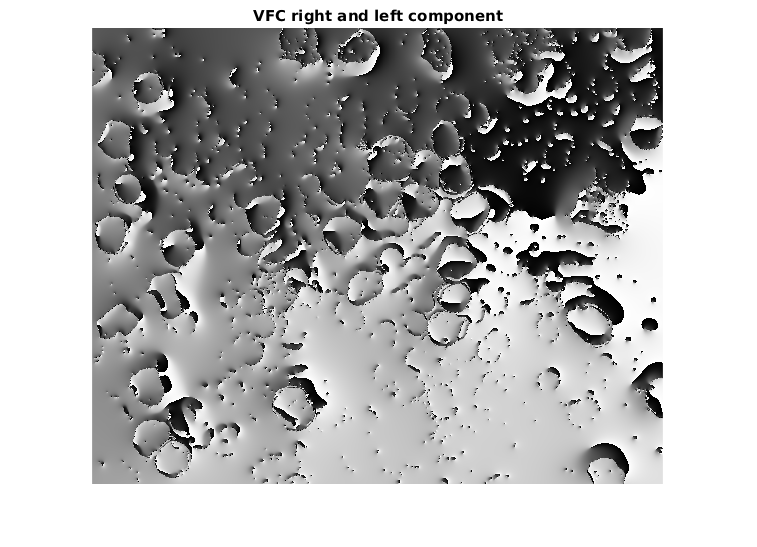
\includegraphics[width=\textwidth]{img/final/figure2.png}
        \caption{ }
        \label{fig:fig}
    \end{subfigure}
    \begin{subfigure}[b]{0.45\textwidth}
        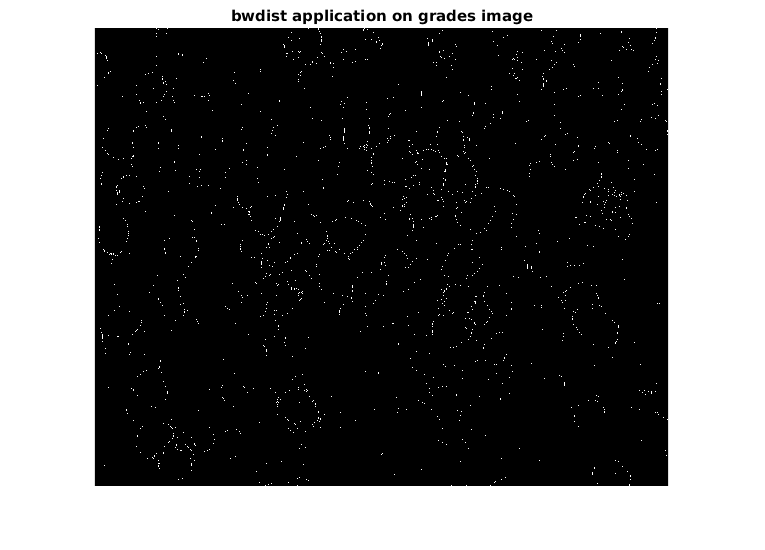
\includegraphics[width=\textwidth]{img/final/figure3.png}
        \caption{ }
        \label{fig:fig3}
    \end{subfigure}
    \begin{subfigure}[b]{0.45\textwidth}
        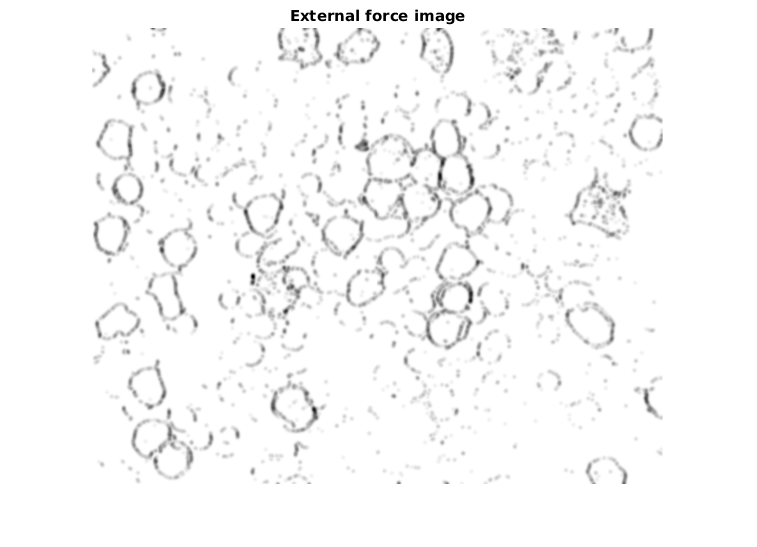
\includegraphics[width=\textwidth]{img/final/figure4.png}
        \caption{ }
        \label{fig:fig4}
    \end{subfigure}
    \begin{subfigure}[b]{0.45\textwidth}
        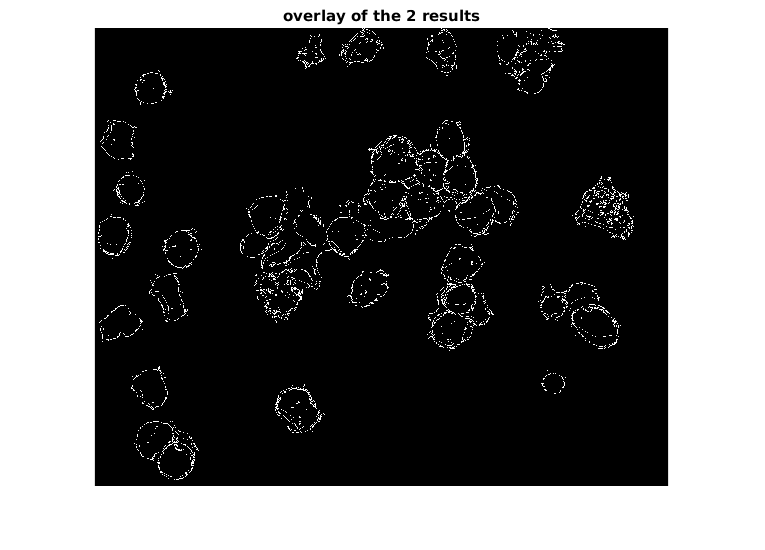
\includegraphics[width=\textwidth]{img/final/figure5.png}
        \caption{ }
        \label{fig:fig5}
    \end{subfigure}
    \begin{subfigure}[b]{0.45\textwidth}
        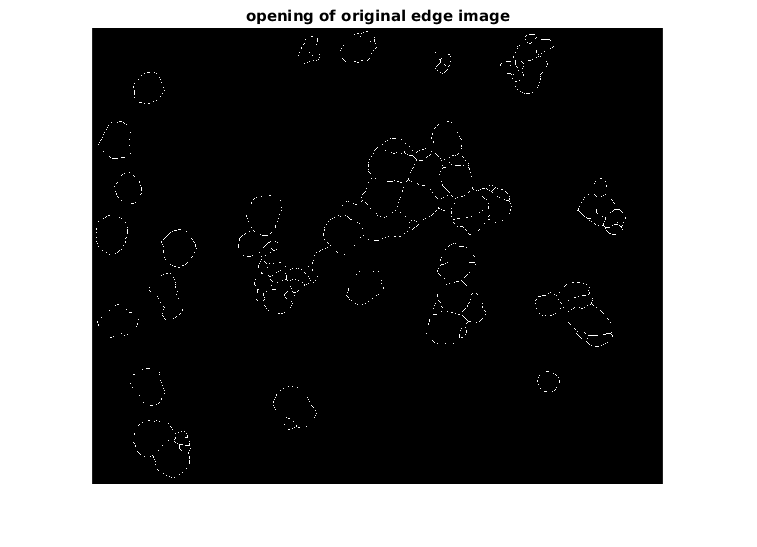
\includegraphics[width=\textwidth]{img/final/figure6.png}
        \caption{ }
        \label{fig:fig6}
    \end{subfigure}
    \begin{subfigure}[b]{0.45\textwidth}
        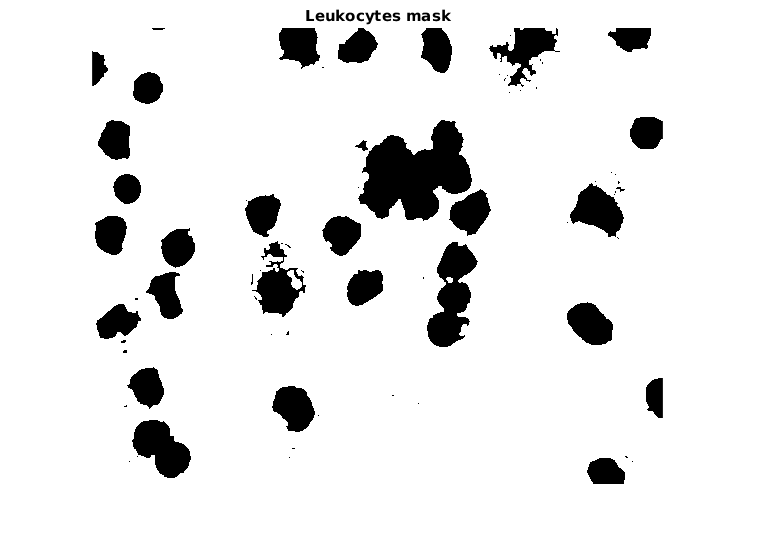
\includegraphics[width=\textwidth]{img/final/figure7.png}
        \caption{ }
        \label{fig:fig7}
    \end{subfigure}

    
    \caption{(a) Mean shift result in gray scale,(b) VFC u and v components,(c) Distance transform on grades image,(d) External force image,(e) Overlay of two results,(f) Opening of initial edge image,(g) Leukocytes mask}
    \label{fig:alltheprocess}
\end{figure}
The last two figures \ref{fig:fig8} \ref{fig:fig9} show the real result of the segmentation.

\begin{figure}
\centering
	\begin{center}
		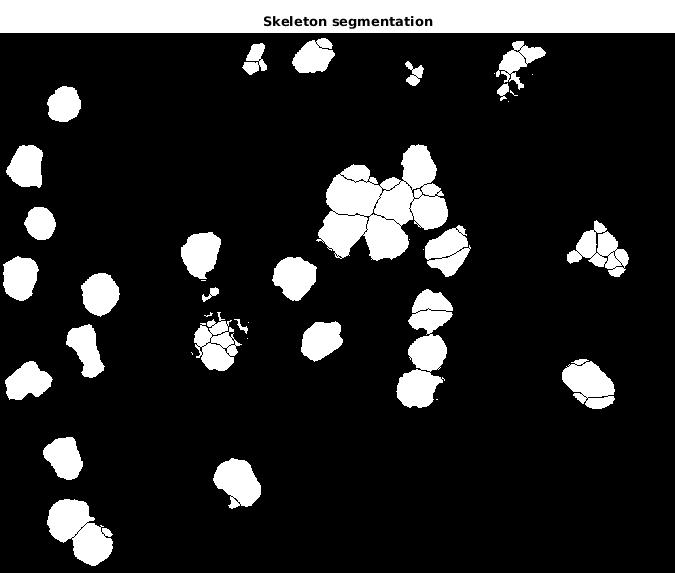
\includegraphics[scale=0.5]{img/final/figure8.png}
		\caption{Skeleton segmentation}
		\label{fig:fig8}
	\end{center}
\end{figure}
\begin{figure}
\centering
	\begin{center}
		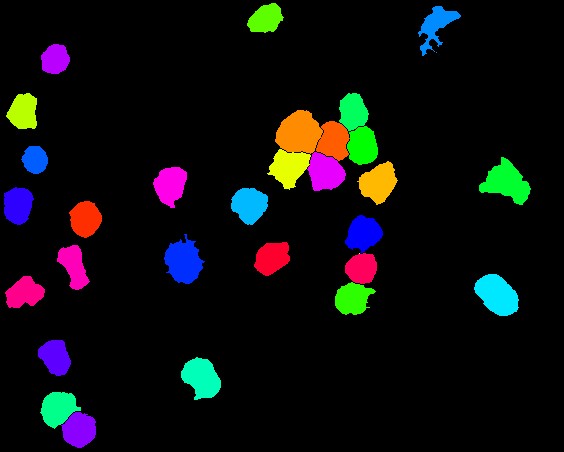
\includegraphics[scale=0.5]{img/final/untitled.png}
		\caption{Merging of little area to count the number of leukocytes}
		\label{fig:fig9}
	\end{center}
\end{figure}
\bigskip
\begin{figure}
\begin{center}
		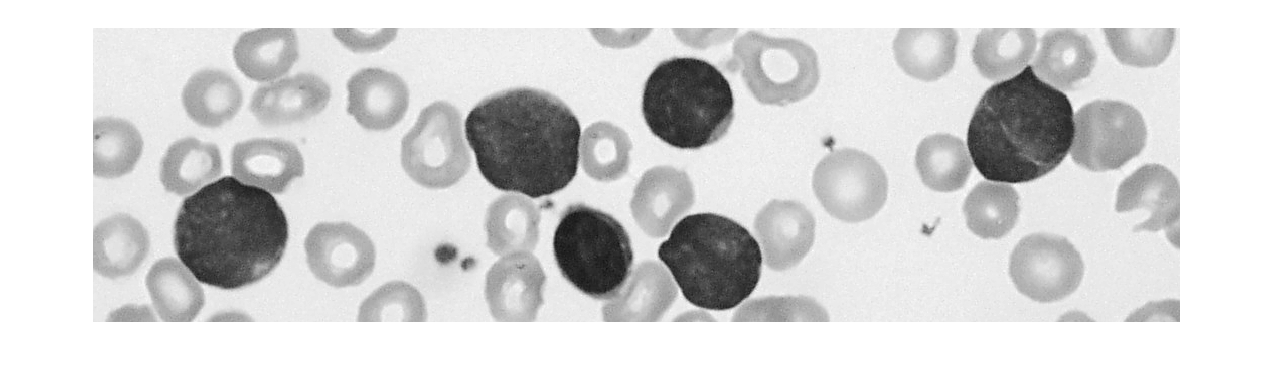
\includegraphics[scale=0.3]{img/final/nooverlap.png}
		\caption{Granulocite after Mean shift application}
		\label{fig:noover}
\end{center}
\end{figure}
\begin{figure}
\begin{center}
		
\includegraphics[scale=0.3]{img/final/nooverlapseg.png}
		\caption{Granulocite after Mean shift application}
		\label{fig:nooverseg}
\end{center}
\end{figure}

As it possible to see, between the two images \ref{fig:fig8} and \ref{fig:fig9} there are some differences. The more visible difference is the bigger presence of agglomerate of small areas that create a kind of cell in the first segmentation. This is happened because it was an artefact caused by the Giemsa stain method, but in our approach we can discriminate all this little areas going to remove them because the over-segmentation of this kind (where there are only little areas) means that isn't a leukocyte but only a stain of colour. The result of the counting in this case is 29. 
Working with cropped images we obtain a better result because we have to analyse less cells and as a consequence we have an increase of the speed as is explained in the table \ref{statistics}.
\begin{table}
\centering
\begin{tabular}{|c|c|c|c|}
\hline 
name & cropped & time & Number of recognized cells / number of real cells\\ 
\hline 
image 5 & no & 45.050214 & 29/29\\ 
\hline 
image 5 & yes & 2.214306 & 7/7\\ 
\hline 
image 13 & no & 31.827737 & 11/11 \\ 
\hline 
image 13 & yes & 1.189616 & 4/4 \\ 
\hline 
image 18 & no & 31.493120 & 18/17\\ 
\hline 
image 18 & yes & 1.717642 & 3/3 \\ 
\hline 
\end{tabular} 
\caption{Statistics result}
\label{statistics}
\end{table}
The table shows only the images where is present the worst case of overlap and clump between the cells. The images where is not present any kind of contact between the cells are well segmented with no problem of over-segmentation. In the images  \ref{fig:noover}, \ref{fig:nooverseg} there is an example of segmentation of six cells without any kind of over-segmentation or division. This is only an example but our implementation works very well with all the images with no overlapped cells. In this case is not useful the mean shift application because the cells are well distant from their selves. This means that the computational cost is very less then the version with the mean shift application (total time $<$ 1 second).

\section{Related works}
Comparing our work with another that obtain the best result using our same dataset \cite{otherwork}, is evident confronting the results where is present a clump or an overlap between the cells that our results are better. In this work the WBC counting is done by counting a number of connected components but is not present a method to divide the clumped cells. We obtain another similar result when we confront our work with a previous work doing in the Cagliari University \cite{dirub}. Also in this work the clumped and the overlapped cells are not well segmented.

\section{Conclusions and future works}
The dissertation proposed an innovative white blood cell recognition and segmentation. It was implemented using some notions already known in literature but never applied in this field. Combining them we obtain a new innovative method in which the major innovation is the use of the Vector field convolution in union to the mean shift and the skeleton function to obtain a result better of the watershed.

\bigskip

The algorithm obtains good results where we analyse images where is not present the granulocyte, because the shape of its nucleus produce a lot of over-segmentation.\ref{fig:grangray}\ref{fig:gran}
\begin{figure}
\begin{center}
		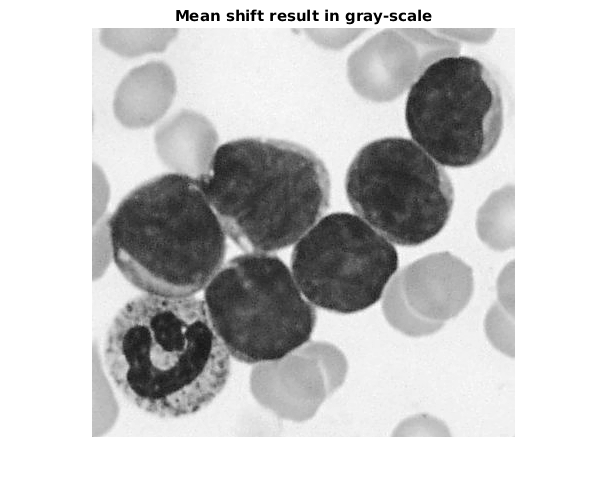
\includegraphics[scale=0.5]{img/final/meangran.png}
		\caption{Granulocite after Mean shift application}
		\label{fig:grangray}
\end{center}
\end{figure}
\begin{figure}
\begin{center}
		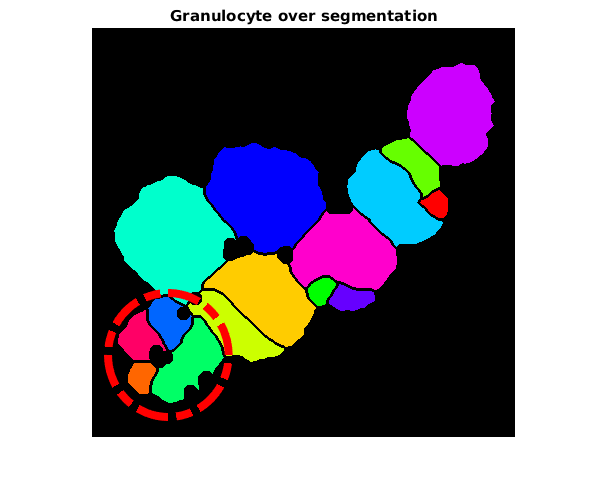
\includegraphics[scale=0.5]{img/final/fingran.png}
		\caption{Over-segmentation caused by the granulocyte}
		\label{fig:gran}
\end{center}
\end{figure}

The most important points that we focused in this thesis can be listed in four sections:
\bigskip

\begin{minipage}{\linewidth}
\begin{enumerate}
\item preprocessing using the mean shift algorithm in order to delete all the differences of colour inside the cells;
\item extrapolation of the right and left component of the VFC force;
\item application of the skeleton in order to separate the overlapped cells;
\item recognize and count of the cells.
\end{enumerate}
\end{minipage}

\bigskip

Our method demonstrates that at this moment is better than everyone algorithm existing in literature. The only problem is the less robustness causing by the low quality images and the over-segmentation caused by the granulocytes. But as the literature says, this is the complex field in histologic image segmentation.

\bigskip

Is possible to resolve this robustness problem. As future works we want to implement a new kind of region merging in order to delete all the over-segmentation caused by the granulocyte and a new points liking function to remove the skeleton side of the algorithm and use only the informations give by the VFC components. 